\clearpage
\subsection{Getting started with MOSL}
\texHeader
\hypertarget{static tex}{} 

\begin{itemize}

\item[$\blacktriangleright$] Create a new metamodel project in Eclipse by navigating to the \texttt{New Metamodel} button in the toolbar. In the dialogue that
appears, enter \texttt{LeitnersLearningBox} as the project name, and select \texttt{Textual (MOSL)}  (Fig.~\ref{fig:new_project}).

\vspace{1cm}

\begin{figure}[htbp]
	\centering
  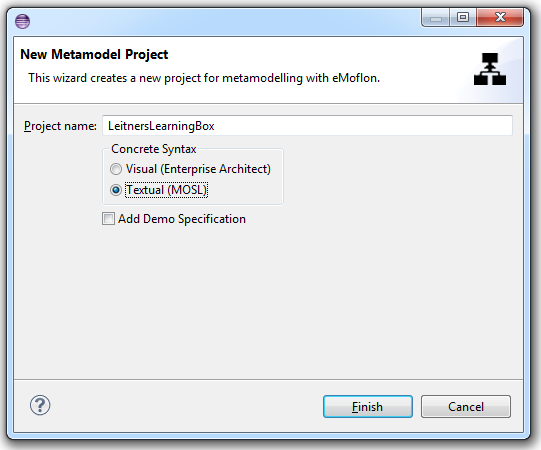
\includegraphics[width=0.8\textwidth]{eclipse_texNewMetamodelPlain}
	\caption{Creating a new metamodel project}
	\label{fig:new_project}
\end{figure}

\vspace{1cm}

\item[$\blacktriangleright$] You'll see your new project appear under the ``Specifications" node.\footnote{If no nodes appear in your package explorer,
make sure your ``Top Level Elements'' are set to ``WorkingSets''} If you're interested in the details on eMoflon's project structure, review section
4.2 from Part I.\footnote{Download link: \dlPartOne} Otherwise, expand the project as deep as it goes (Fig.~\ref{fig:expanded_folders}).

\clearpage

\begin{figure}[htbp]
	\centering
  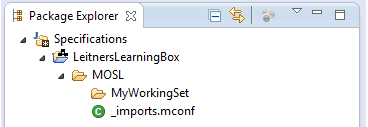
\includegraphics[width=0.6\textwidth]{eclipse_texFoldersExpanded}
	\caption{Expanded project files}
	\label{fig:expanded_folders}
\end{figure} 

\item[$\blacktriangleright$] We're most interested in \texttt{MOSL/MyWorkingSet}, which represents the project scope. Right click this folder, and create a new
\texttt{EPackage} (Fig.~\ref{fig:new_EPackage}), naming it \texttt{LearningBoxLanguage}.

\vspace{0.5cm}

\begin{figure}[htbp]
	\centering
  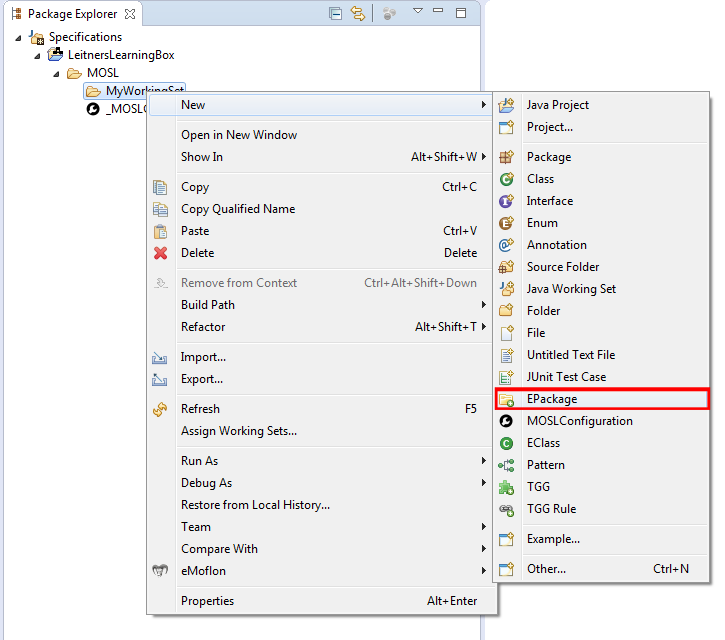
\includegraphics[width=0.8\textwidth]{eclipse_newEPackage}
	\caption{Create an EPackage in your working set}
	\label{fig:new_EPackage}
\end{figure} 

\item[$\blacktriangleright$] Your package explorer should now resemble Fig.~\ref{fig:preBuild}.

\item[$\blacktriangleright$] To finish initalising your metamodel, navigate to ``Build (Without cleaning),'' found beside ``New Metamodel'' in the
toolbar (Fig.~\ref{fig:preBuild}).

\item[$\blacktriangleright$] A new, ``MyWorkingSet'' node, named after your project container, should have been created (Fig.~\ref{fig:finalFiles}). The folder
``gen'' is where all Java files, generated from your metamodel, will be placed.

\clearpage

\begin{figure}[htbp]
	\centering
  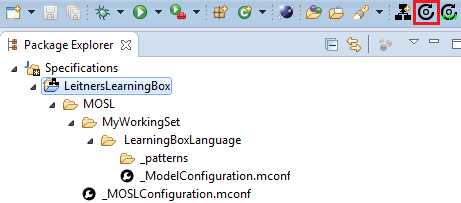
\includegraphics[width=0.6\textwidth]{eclipse_texBuildButton}
	\caption{Inital structure of Leitner's Learning Box}
	\label{fig:preBuild}
\end{figure} 

\vspace{0.5cm}

% Forced position at the bottom of the page
\begin{figure}[h!]
	\centering
  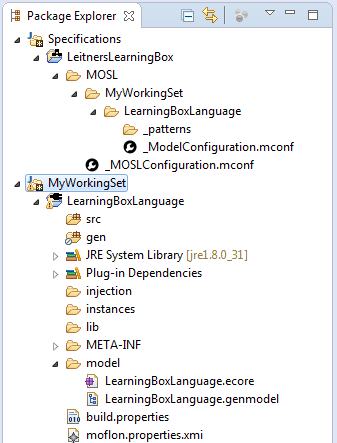
\includegraphics[width=0.5\textwidth]{eclipse_texFinalExpansion}
	\caption{The project fully initialized}
	\label{fig:finalFiles}
\end{figure} 

\vspace{0.5cm}

\item[$\blacktriangleright$] Navigate to ``LearningBoxLanguage/model.'' This folder contains \\ \texttt{LearningBoxLanguage.ecore}, your metamodel. This will
contain all types you define in ``LeitnersLearningBox/MOSL/MyWorkingSet/LearningBoxLanguage.''

\item[$\blacktriangleright$] In the next section, we'll start creating the abstract syntax for Leitner's Box.

\fancyfoot[R]{$\triangleright$ \hyperlink{static:classes tex}{Next}}

\end{itemize}
